
\documentclass[12pt]{article}

\usepackage{algorithm}
\usepackage{algpseudocode}
\usepackage{enumitem}
\usepackage[body={7in,9.5in},centering]{geometry}
\usepackage{fancyhdr}
\usepackage{times}
\usepackage{tikz}
\usepackage{hyperref}
\usepackage{graphicx}

\lhead{}
\rhead{}
\renewcommand{\headrulewidth}{3pt}
\lfoot{}
\cfoot{}
\rfoot{}
\pagestyle{empty}

\newcommand*\circled[1]{\tikz[baseline=(char.base)]{
            \node[shape=circle,draw,inner sep=2pt] (char) {#1};}}


\begin{document}
\begin{center}
  \Large
  CIS 675 (Fall 2018) Disclosure Sheet 
\end{center} 
\vspace*{2em}

\noindent
\textbf{\Large Name: \underline{ Wentan Bai }} 


\noindent 
\begin{minipage}[t]{1.0\linewidth}

\begin{minipage}[t]{0.25\linewidth}
\textbf{\Large
  HW \# \underline{ 4 }
} 

\end{minipage} \vspace*{3ex}




\begin{minipage}[t]{.8in}
  \textbf{\circled{Yes} \quad No}
\end{minipage}
\qquad 
\begin{minipage}[t]{5.5in}
  Did you consult with anyone on parts of this assignment, including other students, TAs, or the instructor? 
\end{minipage}
\vspace*{1ex}

\begin{minipage}[t]{.8in}
  \textbf{\circled{Yes} \quad No}
\end{minipage}
\qquad 
\begin{minipage}[t]{5.5in}
  Did you consult an outside source (such as an Internet forum or a
  book other than the course textbook) on parts of this assignment? 
\end{minipage}
\vspace*{1ex}

\noindent
  If you answered \textbf{Yes} to one or more questions, please give the details here: \vspace*{5ex} \par
  I consulted question 1 and 4 with teaching assistant, Arash Sahebolamri, to confirm my understanding. 
  I also consult all questions and extra question with another student, Wentian Bai. For all questions, we discussed our ideas and I finish my algorithms independently. 

 

\vfill
\end{minipage}



\vspace*{40ex}

By submitting this sheet through my Blackboard account, I assert that the information on this sheet is true.

%\vfill

\hfill {\tiny This disclosure sheet was based on one originally designed
  by
  Profs. Royer and Older.}


\pagebreak
\noindent
\large Question 1: \vspace{5mm} \par
\normalsize 
My algorithm is :
\begin{itemize}
  \item Sort the locations of the paintings in increasing order. The locations of sorted paintings are $l_1$, ..., $l_k$.
  \item	Place one guard at $l_1 + 1$ location, where 1 represent the 1 unit of distance. 
  \item move along the hallway until there is a painting $l_m$ , which is not protected. Place one guard at $l_m + 1$ location.
  \item Repeat the third step until all paintings are protected. 
\end{itemize}

\begin{algorithm}
\begin{algorithmic}
\State \textbf{Sort} locations of the paintings in increasing order \\
\State guard $\leftarrow$ $l_1 + 1$
\State num $\leftarrow$ 1
\State \hspace{0.4cm} \textbf{For} i = 2 to k :
\State \hspace{0.8cm} \textbf{If} guard $<$ $l_i$
\State \hspace{1.2cm} \textbf{} guard $\leftarrow$ $l_i + 1$
\State \hspace{1.2cm} \textbf{} num $\leftarrow$ $num + 1$
\end{algorithmic}
\end{algorithm}
\noindent \\
\textbf{running time:} \par
Sorting uses $O(nlog_{}{n})$ time. We iterate through sorted paintings once using $O(n)$ time.
The final time is $O(nlog_{}{n}) + O(n)$ = $O(nlog_{}{n})$



\pagebreak
\noindent
\large Question 2: \vspace{5mm} \par
\normalsize 
My goal is to maximize the amount of payment. Thus, my idea is trying to schedule the high-paying jobs in the time slot just before their deadline. My algorithm is:
\begin{itemize}
  \item	Sort all jobs by their payments in decreasing order. 
	The sorted jobs are $J_1, J_2, ..., J_m$, and for each job $J_i$, $p_i \leq p_{i+1}$ .
  \item	Schedule $J_1$ in a time slot from time $d_1-1$ to time $d_1$. 
  \item Iterate through the list of remaining jobs in order, and at each step $i$, check whether we can schedule current job $J_i$ from time $d_i-1$ to time $d_i$.
	\begin{itemize}
	\item If this time slot is already scheduled for a job, traverse the timeline forward from time $d_i-1$ and find whether there is a empty slot to schedule current job.
	\item If there is not a empty slot after traversing, we will not schedule this job.
  	\end{itemize}
  \item After going through list, the timeline is expected result. 
\end{itemize}

\begin{algorithm}
\begin{algorithmic}
\State \textbf{Sort} all jobs by their payments in decreasing order.
\State timeline[m] \textbf{ //} m-size array
\State timeline[$d_1$] $\leftarrow$ $J_1$
\State \textbf{For} i = 2 to m :
\State \hspace{0.4cm} \textbf{If} timeline[$d_i$] \textbf{is} empty
\State \hspace{0.8cm} \textbf{}timeline[$d_i$] $\leftarrow J_i$
\State \hspace{0.4cm} \textbf{Else :}
\State \hspace{0.8cm} \textbf{For} k = $d_i-1$ to 1
\State \hspace{1.2cm} \textbf{If} timeline[k] \textbf{is} empty
\State \hspace{1.6cm} \textbf{} timeline[k] $\leftarrow J_i$
\State \textbf{Return} timeline
\end{algorithmic}
\end{algorithm}
\noindent \\
\textbf{running time:} \par
The sorting all jobs uses $O(n\log_{}{n})$. 
When we iterate through sorted jobs, for some jobs, we may need to traverse the timeline forward which uses $O(n)$ time.
Therefore, whole iteration need $O(n^2)$ time. \par
The final time is $O(n\log_{}{n}) + O(n^2) = O(n^2)$


\pagebreak
\noindent
\large Question 3: \vspace{5mm} \par
\normalsize 
I need to consider all possible ways from the first rental shop to the last rental shop. 
Based on dynamic programming, I will record the minimum costs of traversed shop to avoid re-computations. 
My algorithm is:
\begin{itemize}
  \item	Initialize C[1] to 0, which means that there is no cost from first shop to first shop.  
	For other C[2]...C[n], initialize to $c_{1 2} ... c_{1 n}$, 
	which we suppose the cheapest cost from first shop to $i_{th}$ shop is to pick up a canoe at the first rental shop and directly travel to last shop without dropping.
  \item	Using a nested loop to find the cheapest way for each rental shop :
	\begin{itemize}
	  \item For the outer loop, each C[i] represents the cheapest recorded way to get to rental shop $i$.
	  \item Since we have already the cheapest way from first shop to the $i_{th}$ shop, 
		then we use a nested loop to check whether current $C[i] + c_{ij}$ is cheaper than recorded cost to get to rental shop $j$. 
	  \item If current $C[i] + c_{ij}$ is cheaper, update to current cost. Otherwise keep the previous record. 
	\end{itemize}
  \item After iteration, the C[n] records the cheapest cost from first rental shop to last rentail shop. 
\end{itemize}

\begin{algorithm}
\begin{algorithmic}
\State C[n] \textbf{ //} n-size array
\State C[1] $\leftarrow$ $0$
\State \textbf{For} i = 2 to n :
\State \hspace{0.4cm} C[i] $\leftarrow c_{1 i}$ \\

\State \textbf{For} i = 2 to n :
\State \hspace{0.4cm} \textbf{For} j = i + 1 to n :
\State \hspace{0.8cm} \textbf{If} C[j] $>$ C[i] + $c_{ij}$
\State \hspace{1.2cm} C[j] = C[i] + $c_{ij}$ \\
\State \textbf{Return} C[n]
\end{algorithmic}
\end{algorithm}
\noindent \\
\textbf{running time:} \par
The initialization uses $O(n)$ time. 
The whole nested loop needs $O(n^2)$ time. \par
The final time is $O(n) + O(n^2) = O(n^2)$



\pagebreak
\noindent
\large Question 4: \par
\normalsize 
There may be many sets of coins with total value exactly equal to V, but here my goal is to find one. 
My algorithm is:
\begin{itemize}
  \item	Build an array and initialize every element of this array to an empty set. 
	Each set will records only one possible combination of coins. 
  \item	Using a nested loop to find a possible set :
	\begin{itemize}
	  \item For the outer loop, at each step $i$, we only choose the coin with value $v_i$.
	  \item In the inner loop, at each step $j$, check whether we can construct a new set by set[j - $v_i$] $\cup$ $v_i$ exactly equal to value $j$.
	  \item If the new set equals to our expected value $V$, just return it and end loop. 
	\end{itemize}
\end{itemize}

\begin{algorithm}
\begin{algorithmic}
\State n = numbers of coins
\State set[V+1]
\State \textbf{For} i = 0 to V :
\State \hspace{0.4cm} set[i] $\leftarrow$ $\emptyset$ \textbf{ //} every element of this array is an empty set.  \\

\State \textbf{For} i = 0 to n :
\State \hspace{0.4cm} \textbf{For} j = $v_i$ to V :
\State \hspace{0.8cm} \textbf{if} set[j] is $\emptyset$
\State \hspace{1.2cm} set[j] = set[j - $v_i$] $\cup$ $v_i$
\State \hspace{0.8cm} \textbf{if} set[V] is \textbf{not} $\emptyset$
\State \hspace{1.2cm} \textbf{Return} set[V]
\end{algorithmic}
\end{algorithm}
\noindent \\
\textbf{running time:} \par
The initialization uses $O(n)$ time. 
The whole nested loop needs $O(n^2)$ time. \par
The final time is $O(n) + O(n^2) = O(n^2)$




\pagebreak
\noindent
\large Question 5: \par
\large (a): \par
\normalsize 
By hint, sort given boxes by their base area, $W$ $\times$ $L$, in decreasing order. \par
After sorting, we can draw a DAG: 
Establish a nodes i for each box $box_i$, and add direct edge $(i, j)$ whenever it is possible for $box_i$ and $box_j$ whose area is in an decreasing order, 
that is, whenever $i < j$ and $W_i$ $\times$ $L_i$ $>$ $W_j$ $\times$ $L_j$. \par
For example, given 5 boxes :

	\begin{table}[h!]
	  \begin{center}
	    \label{tab:table1}
	    \begin{tabular}{l|c|c|r}
	      \textbf{Box} & \textbf{Width} & \textbf{Length} & \textbf{Height}\\
	      \hline
	      A & 9 & 9 & 1\\
	      B & 7 & 5 & 2\\
	      C & 1 & 2 & 4\\
	      D & 10 & 8 & 2\\
	      E & 2 & 3 & 2\\
	    \end{tabular}
	  \end{center}
	\end{table} \par
The DAG is: \par
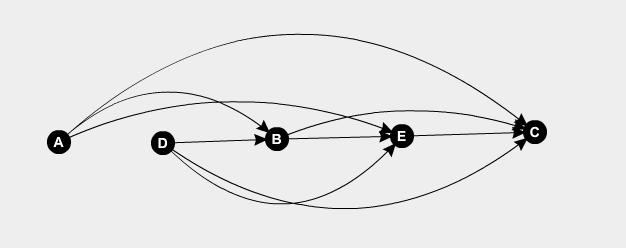
\includegraphics[width=10cm, height=4cm]{question5a} 
\\
\par
Since the constraints, after sorting boxes, every two adjacent boxes can be either stacking or not. And for all $i < j$, $box_j$ can not be on top of $box_i$.
Thus, when we draw a grap, there must be no cycle, which means the graph is DAG.



\pagebreak
\noindent
\large Question 5: \par
\large (b): \par
\normalsize 
My algorithm is:
\begin{itemize}
  \item	sort given boxes by their base area, $W$ $\times$ $L$, in decreasing order.
  \item Create an array $S$ with size of the number of boxes to record the heights of the tallest possible stack for each box.
  \item	Using a nested loop:
	\begin{itemize}
	  \item In the inner loop, since array $S$ records heights of the tallest possible stack of larger boxes, so we traverse $S$ forward to find the maximun S[j] + $H_i$(height of current box). 
	  \item After ending inner loop, we check whether there is a stack is taller than current box. If yes, record height of stack. Otherwise, only record the height of current box. 
	\end{itemize}
  \item Since, there may not be only one smallest box. Thus, at last we iterate through array $S$ and find the maximum one to return.
\end{itemize}

\begin{algorithm}
\begin{algorithmic}
\State Sort given boxes by their base area, $W$ $\times$ $L$, in decreasing order.
\State n = numbers of boxes
\State S[n] \textbf{ //} n-size array
\State \textbf{For} i = 1 to n :
\State \hspace{0.4cm} S[i] $\leftarrow$ 0  \\

\State \textbf{For} i = 1 to n :
\State \hspace{0.4cm} \textbf{}next = 0
\State \hspace{0.4cm} \textbf{For} j = i - 1 to 1 :
\State \hspace{0.8cm} \textbf{if} $W_j$ $\geq$ $W_i$ \textbf{and} $L_j \geq L_i$ \textbf{and} $(H_i+S[j]) > next$ \textbf{:}   
\State \hspace{1.2cm} next = $H_i+S[j]$
\State \hspace{0.4cm} S[i] = max( $H_i$, next)
\\
\State result = S[1]
\State \textbf{For} i = 2 to n :
\State \hspace{0.4cm} \textbf{if} S[i] $>$ result
\State \hspace{0.8cm} \textbf{} result = S[i]
\State result result
\end{algorithmic}
\end{algorithm}
\noindent \\
\textbf{running time:} \par
Sorting need $O(nlog_{}{n})$ time.
The initialization uses $O(n)$ time. 
Therefore, whole iteration need $O(n^2)$ time. \par
The final time is $O(nlog_{}{n}) + O(n) + O(n^2) = O(n^2)$



\pagebreak
\large \textbf{Extra}:\\ \vspace{5mm}\par
\normalsize 
\setlength{\baselineskip}{8mm}

This question is similar as maximum contiguous subsequence. 
Based on description, there are two subseqences which I need to consider:
\begin{itemize}
  \item $x_1 - x_2 + x_3 - x_4 + ... \pm x_n$
  \item $x_2 - x_3 + x_4 - x_5 + ... \pm x_n$
\end{itemize}
Find both sums of maximum contiguous subsequence of above subsequences respectively. The greater one is result.


\begin{algorithm}
\begin{algorithmic}
\State sum1[n]
\State sum1[1] $\leftarrow$ $x_1$
\State \textbf{For} i = 2 to n :
\State \hspace{0.4cm} \textbf{If} i \textbf{mod} 2 == 0 \textbf{:}
\State \hspace{0.8cm} sum1[i] $\leftarrow$ max($x_i$, sum1[$x_{i-1}$] - $x_i$) 
\State \hspace{0.4cm} \textbf{Else}
\State \hspace{0.8cm} sum1[i] $\leftarrow$ max($x_i$, sum1[$x_{i-1}$] + $x_i$)
\\
\State sum2[n-1]
\State sum2[1] $\leftarrow$ $x_2$
\State \textbf{For} i = 3 to n:
\State \hspace{0.4cm} \textbf{If} i \textbf{mod} 2 == 0 \textbf{:}
\State \hspace{0.8cm} sum2[i] $\leftarrow$ max($x_i$, sum2[$x_{i-1}$] + $x_i$) 
\State \hspace{0.4cm} \textbf{Else}
\State \hspace{0.8cm} sum2[i] $\leftarrow$ max($x_i$, sum2[$x_{i-1}$] - $x_i$)
\\
\State firstMax $\leftarrow$ maximum value in sum1
\State secondMax $\leftarrow$ maximum value in sum2
\State \textbf{return} max(firstMax, secondMax)
\end{algorithmic}
\end{algorithm}


\textbf{running time:} \par
Traversing through two subsequences uses $O(n)$ time respectively. Find maximum value in two arrays uses $O(n)$ time respectively. 
Thus my running time is $O(n) + O(n) + O(n) + O(n)$ = $O(n)$.


\end{document} 







